\PassOptionsToPackage{dvipsnames}{xcolor}
\documentclass[]{kw_latex_template}

% single-column: \documentclass[]{bytedance_seed},
%Please prioritize using single-column.

% twocolumn: \documentclass[twocolumn]{bytedance_seed}



%%%%%%%%%%%%%%%%%%%%%%%%%%%%%%%%%%%%

\usepackage{minitoc}
\usepackage{cleveref}
\usepackage{subcaption}
\usepackage{booktabs}
\input{macro}


%%%%%%%%%%%%%%%%%%%%
\renewcommand{\thefootnote}{\fnsymbol{footnote}}

\title{GenericAgent: Self-Evolving LLM Agents with Token-Efficient Context Optimization}
% \author[*]{Jinyi Han$^{1,2}$}
% \author{Zishang Jiang$^{3}$}
% \author{Ying Liao$^{3}$}
% \author{Jiaqing Liang$^{3}$}
% \author[\dagger]{Yanghua Xiao$^{3}$}



% \contribution[*]{Equal Contribution}
% \contribution[\dagger]{Corresponding Authors}

% \affiliation[1]{East China Normal University}

% \affiliation[3]{Fudan University}



\abstract{
Autonomous agents built on large language models face a fundamental bottleneck: as tasks extend over long horizons, redundant and low-value information accumulates within the finite context window, progressively degrading reasoning quality and decision accuracy.
This problem demands a principled approach to managing what information occupies the context at each reasoning step.
We present GenericAgent (GA), a general-purpose LLM agent system designed around the principle of \textbf{context information density maximization}, supporting three complementary operating modes: Interactive, Task, and Reflect, for sustained autonomous operation.
GA makes four main contributions:
(1)~an L0--L3 hierarchical memory architecture that loads information on demand and validates updates through action-level verification;
(2)~a reflection-driven self-evolution mechanism that progressively compresses experiential knowledge from natural-language experience to structured SOPs to executable code and reusable skills;
(3)~a minimal set of seven atomic tools whose principled composition achieves full environmental control;
and (4)~a simplified HTML browser control scheme with incremental DOM monitoring for efficient web interaction.
We release GenericAgent as an open-source system to facilitate research on long-term autonomous agents.

}



\begin{document}

\maketitle

\section{Introduction}
Large language model (LLM) based autonomous agents have advanced rapidly in recent years, demonstrating remarkable capabilities in code generation, web browsing, and complex task automation~\cite{react,cot,gpt4}.
Systems such as Claude Code~\cite{claudecode}, Codex~\cite{codex}, and OpenHands~\cite{openhands} can now interpret high-level instructions and execute multi-step plans that span dozens of tool invocations.
Yet the vast majority of these systems are architected for \emph{single-session} task completion: an agent receives a request, carries it out, and terminates without retaining any knowledge for future sessions.
This design assumption breaks down when agents are expected to operate autonomously over extended time horizons---managing personal workflows, monitoring evolving environments, or accumulating domain expertise across hundreds of interactions.
In such long-term settings, the context window becomes the fundamental bottleneck rather than model capability itself~\cite{anthropic_context}.
Tool definitions, historical memory, retrieved documents, and raw web content all compete for the same finite token budget, continuously expanding the prompt while squeezing the space available for effective reasoning.
Empirical evidence consistently shows that, given the same informational requirements, longer prompts degrade model performance: attention becomes diluted, irrelevant tokens introduce noise, and critical instructions are more likely to be overlooked.
This tension between the growing information demands of long-term operation and the fixed capacity of the context window constitutes the central challenge that motivates our work.

We identify four concrete dimensions along which context information density is eroded in existing agent systems, each representing a distinct source of what we term \emph{context pollution}.
First, \textbf{memory retrieval}: as an agent accumulates knowledge across sessions, its memory store grows without bound, yet each decision typically requires only a small, precise subset of that knowledge---retrieving too much wastes context, while retrieving too little causes the agent to forget critical facts.
Second, \textbf{experience reuse}: when an agent encounters a task similar to one it has solved before, the ideal behavior is to leverage prior experience; however, raw reasoning traces are verbose, filled with exploratory dead ends and redundant deliberation that are costly to re-inject into the prompt.
Third, \textbf{tool overhead}: standard agent frameworks inject the full schema of every available tool into the system prompt on every LLM call, imposing a persistent, per-turn token cost that scales linearly with the size of the tool library~\cite{react}.
Fourth, \textbf{web interaction}: when agents browse the web, raw HTML pages contain navigation bars, advertisements, scripts, and boilerplate that vastly outnumber the task-relevant content, yet conventional approaches pass this entire payload to the model.
Existing systems have addressed these challenges in isolation---MemGPT~\cite{memgpt} proposes OS-inspired virtual memory but lacks mechanisms for self-evolution, Voyager~\cite{voyager} introduces a skill library but is confined to Minecraft, and multi-agent architectures such as Manus~\cite{manus} distribute complexity across specialized sub-agents without fundamentally reducing per-agent context consumption.
No prior system has addressed all four dimensions under a unified design principle.

In this paper, we present \textbf{GenericAgent}, a general-purpose LLM agent system designed from the ground up around the principle of \emph{context information density maximization}: within the finite context window available to each LLM call, the system should pack the highest-density, most task-relevant information so as to maximize the probability of task success while minimizing total prompt cost.
The corollary of this principle is equally important: when the information required for a decision is already complete, a shorter prompt will yield better performance than a longer one, because every superfluous token is a source of distraction rather than signal.
GenericAgent instantiates this principle through four tightly integrated subsystems---hierarchical memory, reflection-driven self-evolution, minimal atomic tools, and context-compressed browser control---each targeting one of the four information density challenges identified above.
All subsystems are unified under a single \emph{Agent Loop} that drives three complementary operating modes: \textbf{Interactive} mode for direct user commands, \textbf{Task} mode for sub-agent coordination via structured file I/O, and \textbf{Reflect} mode for event- or cron-triggered autonomous operation.
The entire system is implemented in approximately 3,000 lines of core code, supports multiple LLM backends including Claude, OpenAI, and Gemini, and is publicly available at \url{https://github.com/lsdefine/GenericAgent}.

Our main contributions are as follows:
\begin{itemize}[leftmargin=*]
    \item A \textbf{hierarchical memory system} (L0--L3) with taxonomy-based indexing and action-verified updates, ensuring that only the minimal, validated information needed for each decision is retrieved into the context window.
    \item A \textbf{reflection-driven self-evolution} mechanism that progressively compresses raw experience into standard operating procedures, then into executable code, and ultimately into composable skills---each stage reducing the context cost of reusing past knowledge by an order of magnitude.
    \item A set of \textbf{seven minimal atomic tools} whose compact definitions occupy a fraction of the prompt budget consumed by conventional tool libraries, yet achieve full environmental control through principled composition~\cite{reflexion}.
    \item A \textbf{context-compressed browser control} scheme based on simplified HTML rendering and incremental DOM monitoring, which strips web pages down to their task-relevant semantic content before injection into the context window.
\end{itemize}


\section{GenericAgent}
\begin{figure*}[t]
    \centering
    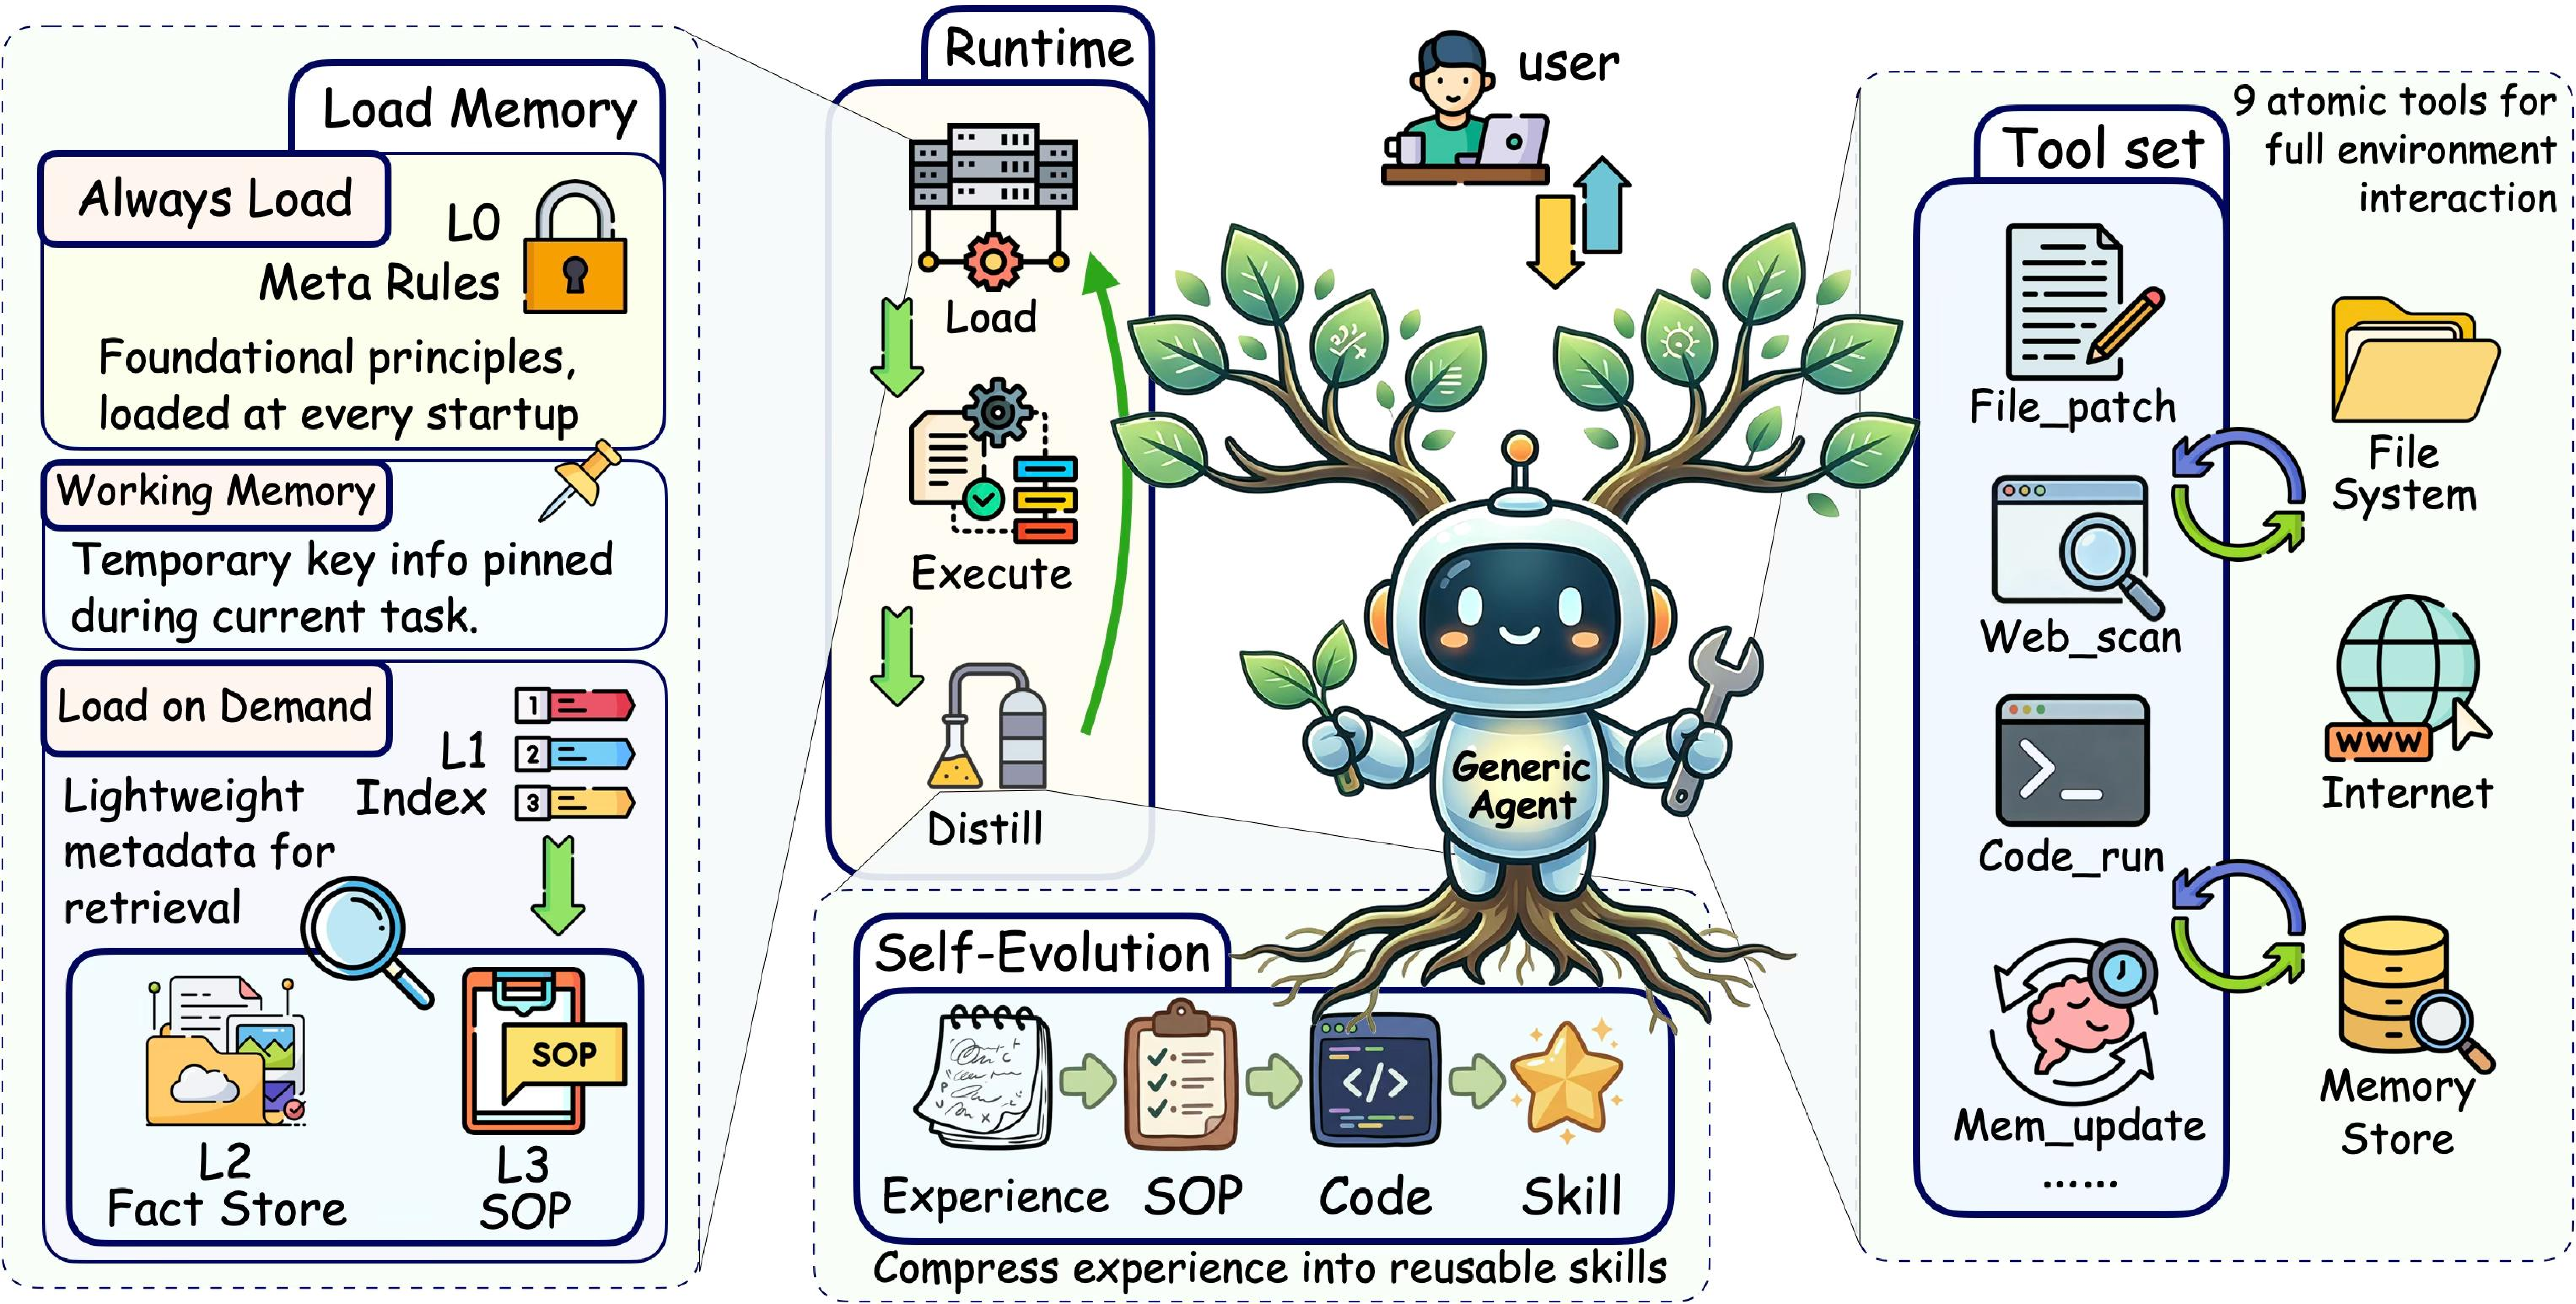
\includegraphics[width=0.98\linewidth]{image/framework_0413.pdf}
    \caption{\textbf{Overall framework of GA.}}
    \label{fig:agent_loop}
\end{figure*}

\subsection{Design Principles}
\label{sec:principle}
\begin{AIbox}
GA is designed around the principle of \textbf{maximizing contextual information density}. The goal is to provide the most decision-relevant information within a limited context budget.
\end{AIbox}

GA aims to maximize decision-relevant information under a fixed context budget. In practice, the performance of LLM agents depends not only on context length, but also on how context is organized. Redundant content diffuses attention. Irrelevant history interferes with the current task. Overly compressed representations can hide useful structure and reduce interpretability. These issues all lower information density. To address them, GA requires contextual content to satisfy three constraints:
\begin{itemize}
    \item \textbf{Completeness.} {\small
    All information required for the current decision should be explicitly available in context, so the model does not rely on missing premises or unsupported completion.
    }

    \item \textbf{Conciseness.} {\small
    Irrelevant and redundant content should be removed, so attention remains focused on decision-critical signals.
    }

    \item \textbf{Naturalness.} {\small
    Context should remain in clear and well-formed natural language, so semantic structure is preserved and the content remains easy to interpret.
    }
\end{itemize}

These constraints are complementary. Completeness prevents missing information. Conciseness removes non-essential content. Naturalness preserves interpretability. Together, they define a contextual representation that is both information-rich and tractable for reasoning.

Based on these constraints, GA is organized around four principle-level mechanisms: tool minimality, hierarchical memory, reflection-driven adaptation, and structured browser extraction. The following subsections introduce these mechanisms conceptually. Section~\ref{sec:core_design} then presents their concrete design in detail.

\subsubsection{Tool Minimality}
% In agent-loop systems, tool definitions are typically injected into the context at each model call. Tool design therefore contributes directly to contextual overhead. GA addresses this issue with a small set of atomic tools designed for composition. This design favors irreducible primitives over task-specific interfaces, so complex tasks can be expressed through short tool sequences rather than a large tool inventory.
In existing agent loop architecture, tool definitions are explicitly injected into the context at every LLM call, making tool design a key determinant of context information density. To reduce the overhead introduced by tool schemas, GA adopts a minimal tool set consisting of nine atomic tools and follows two core principles: \textbf{atomicity} and \textbf{compositional generalization}. Atomicity constrains tool granularity by enforcing irreducible primitive capabilities, while compositional generalization enables the expression of complex tasks through sequential composition of these atomic tools. Table~\ref{tab:tools} summarizes the complete GA tool set.

This minimal tool set yields two direct benefits. First, it significantly reduces tool-description overhead in the context. In multi-turn interactions, a smaller and more interface-efficient tool set directly reduces cumulative token consumption across calls. Second, it reduces the model’s decision complexity. A compact and well-bounded action space decreases uncertainty in tool selection, enabling more stable tool-use patterns and thereby reducing execution errors and retries.

Besides, GA does not rely on specialized tools to expand functionality. Instead, complex behaviors are composed from atomic primitives. For example, file-level operations follow a standard read–modify–write paradigm, while web interactions are decomposed into content retrieval and browser-side execution. External capabilities are encapsulated as Skills and invoked indirectly through general-purpose code-execution and web-related primitives, and are loaded into the context only on demand. 

\subsubsection{Hierarchical Memory}
% GA retains only information that is difficult to reconstruct from the current context or from direct reasoning. It filters redundant signals and preserves only information that can meaningfully affect future behavior. This keeps memory compact and behaviorally useful.

GA retains only information that cannot be readily reconstructed from the current context or inferred by the model through reasoning. It aggressively filters out redundant signals and preserves only experience that introduces non-trivial behavioral change. The objective is to maximize the marginal impact of each retained interaction on future decisions, ensuring that stored experience directly shapes and improves GA's behavior.

The memory system follows a four-layer architecture with hierarchical distillation and taxonomy-based organization. It focuses on keeping only behaviorally useful knowledge. L0 defines constraints. L1 handles routing. L2 stores verified facts. L3 captures reusable experience. Together, they allow GA to operate within a fixed context budget while maximizing the utility of each token.

\subsubsection{Reflection-Driven Adaptation}
GA’s self-evolution mechanism is an abstraction-driven process that compiles execution trajectories into high-density reusable representations. It preserves semantic integrity while reducing reasoning cost. Through periodic reflection, GA analyzes historical execution traces and converts them into structured knowledge. These structures are then organized into executable forms. The evolution is guided by user task distributions and behavioral patterns, ensuring alignment with real-world usage and observed failures.

\subsubsection{Structured Browser Extraction}
GA treats browser interaction as structured extraction of task-relevant information rather than full-page retrieval. Raw web pages contain large amounts of irrelevant DOM content, which increases token cost without proportional utility. GA therefore extracts compact page representations that preserve task-relevant signals while controlling context growth.

\subsection{System Overview}
\label{sec:overview}
GA is a general-purpose LLM agent system for local computer automation. It enables a compatible model backend to interact with browsers, terminals, file systems, keyboard and mouse input, screen-based perception, and mobile devices through configurable tool adapters. The system is model-agnostic: the underlying model can be replaced without changing the execution loop, tool interfaces, or memory architecture. Figure~\ref{fig:agent_loop} illustrates the overall framework.

GA operates through a unified agent loop that connects the model and the environment. At each step, the system combines the current task with relevant memory to form the execution context. The model then produces either a direct response or a tool call. External modules execute tool calls and return structured results, which update the system state for the next step. This loop supports iterative, tool-grounded interaction.

On top of this loop, GA supports two execution modes. \textbf{Interactive execution} handles user-initiated tasks such as file operations, information retrieval, and code execution. \textbf{Reflective execution} runs in the background and is triggered by schedules or system events. It is used for monitoring, memory consolidation, and experience distillation. The two modes share the same execution loop and memory system, but differ in how they are initiated and how their outputs are consumed. GA also enforces explicit execution bounds to preserve controllability, interruptibility, and task scope.

After task completion, GA distills execution traces into structured long-term representations and stores them in shared memory. These representations can be reused across both execution modes, allowing the system to improve through compression and reuse.

\subsection{Core Components of GA}
\label{sec:core_design}
We now describe the concrete design of the four mechanisms introduced above: the minimal atomic toolset, the hierarchical memory architecture, reflection-driven self-evolution, and structured extraction for efficient browser interaction.

\subsubsection{Minimal Atomic Toolset}
\label{sec:tools}
GA’s tool system is designed to achieve broad computer operation coverage with a minimal set of atomic tools. Instead of expanding tools according to task needs, it abstracts them along underlying capability boundaries, which prevents toolset bloat and ensures long-term stability and composability. Concretely, GA compresses all capabilities into five core dimensions: file system, browser, code execution, human-in-the-loop interaction, and memory management. Within each dimension, only the minimal necessary atomic operations are retained, allowing tools to directly correspond to fundamental OS and browser behaviors rather than task-specific abstractions, thereby enabling cross-task generality.

GA strictly aligns each tool with physical execution boundaries. The file system exposes only read, write, and patch-style differential modification, while the browser exposes only DOM inspection and JavaScript execution. More complex behaviors are delegated to scripts or multi-step compositions, avoiding high-level semantic APIs and ensuring consistency with real system semantics.

GA adopts an atomic-tool plus sequential-composition paradigm, where each tool performs a single, well-defined primitive action, and complex tasks are completed through tool chaining. This design deliberately shifts complexity from the tool layer to the reasoning and planning layer, rather than introducing increasingly specialized or “fat” tools.

Safety and auditability are enforced directly at the interface level. Write operations are explicitly separated into overwrite and patch-based updates, critical modifications require exact content matching, and irreversible actions must be confirmed through human-in-the-loop interaction. Long-term state updates are also triggered through an explicit memory update mechanism, preventing uncontrolled global state modifications during execution.

At the interface level, GA maintains lightweight and human-readable tool calls. JSON arguments are restricted to metadata such as paths, modes, and flags, while large payloads such as code or structured content are carried in readable blocks. This design improves both machine executability and human debuggability.

Overall, GA builds an extremely compact tool system through capability compression and physical boundary alignment. It relies on atomic composability rather than tool proliferation, making system extensibility depend on tool sequence planning rather than toolset expansion.

\begin{table}[t]
    \centering
    \caption{Atomic tools in GA.}
    \label{tab:tools}
    {\footnotesize
    \setlength{\tabcolsep}{3pt}
    \renewcommand{\arraystretch}{0.95}
    \begin{tabularx}{\linewidth}{@{}lX@{}}
    \toprule
    \textbf{Tool} & \textbf{Brief Description} \\
    \midrule
    \texttt{code\_run} &
    Execute Python or shell code with timeout and abort control. \\
    \texttt{file\_read} &
    Read local files by line range, with optional keyword-based lookup. \\
    \texttt{file\_write} &
    Create files or write large content blocks in overwrite, append, or prepend mode. \\
    \texttt{file\_patch} &
    Apply precise, context-checked updates to existing file regions. \\
    \texttt{web\_scan} &
    Extract the current browser page as simplified HTML or text, together with tab metadata. \\
    \texttt{web\_execute\_js} &
    Inject and execute JavaScript in the user’s browser and capture the return value. \\
    \texttt{ask\_user} &
    Issue a synchronous query to the user and wait for an explicit response. \\
    \shortstack[l]{\texttt{update\_working\_}\\\texttt{checkpoint}} &
    Update a short-term working note that is injected into subsequent reasoning turns. \\
    \shortstack[l]{\texttt{start\_long\_term\_}\\\texttt{update}} &
    Trigger long-term memory distillation over recent execution traces. \\
    \bottomrule
    \end{tabularx}
    }
\end{table}

\subsubsection{Hierarchical Memory Architecture}
\label{sec:memory}
GA follows a four-layer architecture with hierarchical distillation and taxonomy-based organization.

\textbf{L0: Meta-Rule Layer.}  L0 defines the core behavioral constraints of GA. It acts as a lightweight control layer for system operation and self-regulation. Each rule is written in a single sentence. For example: ``Only information verified through execution can be written to long-term memory.'' This rule prevent unverified or hallucinated information from entering long-term memory. L0 is injected into the system prompt at startup with minimal overhead and remains fixed during execution.

\textbf{L1: Index Layer.} L1 provides a lightweight index for memory routing. It stores only metadata, file paths, short descriptions, and applicability conditions. It does not store full content.

Before each task, GA queries L1 and retrieves only relevant memory entries. This keeps the active context sparse even as the memory base grows. The L1 index is maintained at around 30 lines, keeping retrieval overhead low.

\textbf{L2: Fact Store.}  L2 stores verified environmental facts. It includes information that cannot be easily inferred, such as directory structures, configurations, API endpoints, and system constraints.

All entries are validated through tool execution or external signals. Information is organized by topic and incrementally summarized. This reduces fragmentation and improves retrieval clarity.

\textbf{L3: Task-Level SOP Layer.} L3 stores reusable task-level procedures. It captures patterns such as tool usage order, dependencies, failure cases, and correction strategies.

These SOPs are extracted from execution traces after task completion. They are not manually written. In later tasks, a small amount of L3 content can guide behavior and improve success rates.

\subsubsection{Reflection-Driven Self-Evolution}
\label{sec:self-evolution}
GA is not a fixed prompt wrapped around a model. It is an agent system whose internal behavior is continuously shaped by execution, while its external interface remains stable and minimal.

During task execution, GA transforms raw execution traces into \textbf{structured representations} of its own decisions, rather than leaving them as unorganized dialogue history. As similar tasks recur, these representations are progressively distilled and compressed into reusable strategies and executable skills, enabling future problem solving to rely less on repeated ad-hoc reasoning and more on internal skill composition. This reduces redundant reasoning over time, leading to lower token consumption in repeated or structurally similar tasks. Specifically, this mechanism consists of three stages.

\textbf{Stage 1: Experience Distillation into SOPs.} GA analyzes historical execution traces to extract useful information, including successful decision paths and failure patterns. These are abstracted into SOPs that describe stable execution logic.

This stage serves two purposes. First, it generalizes instance-level behavior into reusable process specifications. Second, it prioritizes high-frequency and high-error tasks. Routine or low-impact steps are discarded to improve compression and generalization.

\textbf{Stage 2: SOP Compilation into Code.} SOPs with stable structure are evaluated for compilation. If a task shows clear parameterization, deterministic logic, and explicit dependencies, it is converted into code.

This replaces procedural reasoning with program execution. Execution becomes structured and deterministic. Compared to SOPs, code provides clearer semantics and more stable behavior under repeated execution.

\textbf{Stage 3: Registration as Skills.} Compiled code modules are registered as Skills in GA’s indexing system. Skills are reusable execution units. Similar tasks can directly invoke them, without intermediate reasoning.

GA monitors Skill usage and updates implementations over time. Updates include interface simplification, parameter refinement, and execution optimization. This improves efficiency per token.

These stages form a closed loop. Reflection extracts experience, SOPs generalize behavior, code replaces reasoning, and Skills enable reuse. This process improves efficiency over time and reduces redundant computation. 

\subsubsection{Structured Extraction for Efficient Browser Interaction}
Interacting with web pages is expensive in tokens. A full DOM often contains tens of thousands of tokens, while only a small portion is useful for the current task. Sending the full DOM to the model is not practical. At the same time, aggressive filtering may remove important signals. GA address this with a two-stage extraction pipeline.

\textbf{Geometry-aware DOM pruning.} A JavaScript routine clones the DOM with access to layout information. Invisible nodes are removed, including hidden elements, zero-area nodes, and off-screen content. Modal dialogs and cookie banners are explicitly detected by their viewport coverage and moved to the top level. Form states such as input values and checkboxes are preserved during cloning. This ensures the snapshot matches the actual visible page state.

\textbf{Token-budget compression.} The pruned DOM is further compressed using structural filtering. Non-semantic attributes are removed. URLs are shortened. Decorative metadata is dropped. The page structure is preserved, but the token cost is greatly reduced. Large list structures are handled separately. The system detects lists using layout regularity and structural signals. Only a small number of representative items are kept. The rest are replaced with a placeholder that records the approximate size and content pattern. This keeps the structure while avoiding full expansion.

When the result still exceeds the token budget, a recursive truncation step is applied. The reduction is distributed across subtrees instead of using a flat cutoff. This preserves global structure.

After each browser action, GA does not re-read the full page. Each action is wrapped with a pre- and post-state snapshot. The model receives only the diff and transient UI signals such as toasts or loading indicators. This reduces redundant observation and tightens the interaction loop.











\section{Experiments}

\subsection{Experimental Setup}
\label{sec:exp_setup}

\paragraph{Evaluation Objectives.}
Our experiments are designed to validate the core claims of GenericAgent across six dimensions:
(1) whether the memory system enables continuous efficiency improvement over repeated tasks,
(2) whether condensed memory achieves better cost-effectiveness than full or redundant memory,
(3) whether the self-evolution mechanism progressively reduces execution cost,
(4) tool usage efficiency in real-world scenarios,
(5) autonomous web browsing capability on diverse websites,
and (6) robustness against indirect prompt injection and malicious instructions.

\paragraph{Baselines.}
We compare GenericAgent (GA) against three representative agent systems:
\textbf{Claude Code}~\cite{claudecode}, a production-grade coding assistant with built-in memory and skill management;
\textbf{Codex}~\cite{codex}, OpenAI's code-generation agent;
and \textbf{OpenClaw}~\cite{openclaw}, an open-source general-purpose agent framework.
All systems use the same backbone LLM (GPT-5.4 or Claude Opus 4.6, specified per experiment) to ensure fair comparison.

\paragraph{Implementation Details.}
GenericAgent is implemented in Python with approximately 3,000 lines of core code.
The hierarchical memory system maintains an L1 index capped at 30 entries (~1,000 tokens).
The agent loop enforces a maximum of 40 reasoning turns per task, with warnings issued every 7 turns and forced user confirmation at turn 35.
Browser control uses TMWebDriver with dual-channel communication (WebSocket on port 18765, HTTP long-polling on port 18766).
All experiments are conducted on a standard development workstation with 32GB RAM and an Intel i9 processor.


\subsection{Memory System Effectiveness}
\label{sec:exp_memory}

\subsubsection{Continuous Efficiency Improvement}

A key claim of GenericAgent is that it gets better with use---each task execution should leave behind distilled knowledge that accelerates future similar tasks.
To test this, we repeatedly execute the same type of task across multiple sessions: downloading five different datasets from HuggingFace.
Each download runs in a fresh session to prevent context carryover, and we measure operation time (excluding actual download duration) and token consumption.

Table~\ref{tab:memory_improvement} reveals a striking divergence between GenericAgent and the baselines.
CodeX, Claude Code, and OpenClaw exhibit stable performance with minor fluctuations---no learning occurs across sessions.
GenericAgent, however, shows continuous improvement: the first task requires 102s and 200,439 tokens, but by the fourth task, operation time drops to 62s (39.2\% reduction) and by the fifth task, token consumption falls to 99,382 (50.4\% reduction).

\begin{table}[t]
\centering
\caption{Performance evolution across five HuggingFace download tasks. GenericAgent shows continuous improvement while baselines remain stable.}
\label{tab:memory_improvement}
\begin{tabular}{lcccccc}
\toprule
\textbf{System} & \textbf{Task 1} & \textbf{Task 2} & \textbf{Task 3} & \textbf{Task 4} & \textbf{Task 5} & \textbf{Improvement} \\
\midrule
\multicolumn{7}{l}{\emph{Operation Time (seconds)}} \\
\midrule
CodeX & 95 & 98 & 92 & 97 & 94 & -1.1\% \\
Claude Code & 88 & 91 & 89 & 93 & 90 & +2.3\% \\
OpenClaw & 112 & 108 & 115 & 110 & 113 & +0.9\% \\
GenericAgent & 102 & 78 & 71 & 62 & 65 & \textbf{-39.2\%} \\
\midrule
\multicolumn{7}{l}{\emph{Token Consumption}} \\
\midrule
CodeX & 185,234 & 188,921 & 182,445 & 190,332 & 186,778 & +0.8\% \\
Claude Code & 172,889 & 175,234 & 170,992 & 178,445 & 174,223 & +0.8\% \\
OpenClaw & 215,667 & 218,934 & 212,445 & 220,112 & 217,889 & +1.0\% \\
GenericAgent & 200,439 & 145,223 & 128,667 & 112,334 & 99,382 & \textbf{-50.4\%} \\
\bottomrule
\end{tabular}
\end{table}

This improvement stems from memory distillation: after the first task, key steps and common pitfalls are extracted into L3 SOPs.
Subsequent executions leverage this accumulated knowledge, bypassing redundant reasoning and avoiding repeated errors.
Baseline systems, lacking systematic memory consolidation, treat each task as independent and fail to capitalize on prior experience.


\subsubsection{Condensed vs. Full Memory}

Our memory system prioritizes information density over completeness, but does this actually improve performance?
We test this on the SOP-Bench dangerous\_goods subset, which requires strict adherence to procedural rules.
Four memory configurations are compared: \textbf{No-Memory} (no external knowledge), \textbf{Condensed-Memory} (minimal critical rules only), \textbf{Full-Memory} (complete SOP documentation), and \textbf{Redundant-Memory} (condensed memory plus background explanations).
All use GPT-5.4 and are evaluated on Task Success Rate (TSR).

The results in Table~\ref{tab:memory_ablation} are counterintuitive.
No-Memory achieves only 13.87\% TSR, confirming that external procedural knowledge is essential.
But Full-Memory, despite containing all relevant information, reaches only 52.44\% TSR---significantly worse than both Condensed-Memory and Redundant-Memory (66.48\%).
More striking: Condensed-Memory uses only 165 tokens (28.7\% of Full-Memory's 575 tokens) yet matches Redundant-Memory's performance at 57.3\% of its cost.

\begin{table}[t]
\centering
\caption{Memory ablation on SOP-Bench dangerous\_goods. Condensed memory achieves the best cost-effectiveness.}
\label{tab:memory_ablation}
\begin{tabular}{lcc}
\toprule
\textbf{Configuration} & \textbf{Memory Size (tokens)} & \textbf{TSR (\%)} \\
\midrule
No-Memory & 0 & 13.87 \\
Full-Memory & 575 & 52.44 \\
Redundant-Memory & 288 & 66.48 \\
Condensed-Memory & 165 & \textbf{66.48} \\
\bottomrule
\end{tabular}
\end{table}

This validates our core principle: effective memory is not about completeness but about \emph{criticality}.
Full-Memory includes extensive background and definitions that dilute attention without improving decision quality.
Condensed-Memory retains only the rules that directly alter model behavior, achieving superior performance at minimal cost.
The equivalence between Condensed-Memory and Redundant-Memory confirms that additional explanatory content provides no marginal benefit.


\subsubsection{Long-Term Fact Retention}

Long-term memory systems typically rely on vector databases and embedding-based retrieval.
GenericAgent takes a different approach: hierarchical organization with action-verified updates, no embeddings required.
We test whether this simpler architecture can compete on the Locomo10 benchmark (excluding Category 5 Summary tasks).
The remaining categories---Multi-Hop, Temporal, Open-Domain, and Single-Hop---test recall and reasoning over stored facts.
Baselines include Mem0 and A-MEM (both using text-embedding-3-small) and OpenClaw (no embedding model), all with GPT-5.4 backbone.

Table~\ref{tab:long_term_memory} shows GenericAgent outperforming all baselines across all four categories, despite its simpler architecture.
The advantage is most pronounced in Multi-Hop (F1: 43.33 vs. 39.32 for Mem0) and Temporal (F1: 52.23 vs. 50.03) tasks, suggesting strong cross-fact reasoning.
Even in the challenging Open-Domain category, where all systems struggle, GA maintains a lead (F1: 20.41 vs. 18.32).

\begin{table}[t]
\centering
\caption{Long-term factual memory evaluation on Locomo10. GenericAgent outperforms embedding-based systems without using external retrieval.}
\label{tab:long_term_memory}
\begin{tabular}{lcccccccc}
\toprule
& \multicolumn{2}{c}{\textbf{Multi-Hop}} & \multicolumn{2}{c}{\textbf{Temporal}} & \multicolumn{2}{c}{\textbf{Open-Domain}} & \multicolumn{2}{c}{\textbf{Single-Hop}} \\
\cmidrule(lr){2-3} \cmidrule(lr){4-5} \cmidrule(lr){6-7} \cmidrule(lr){8-9}
\textbf{System} & \textbf{F1} & \textbf{BLEU} & \textbf{F1} & \textbf{BLEU} & \textbf{F1} & \textbf{BLEU} & \textbf{F1} & \textbf{BLEU} \\
\midrule
Mem0 & 39.32 & 28.43 & 50.03 & 43.33 & 18.32 & 13.80 & 40.32 & 32.33 \\
A-MEM & 29.03 & 20.48 & 46.83 & 38.84 & 13.11 & 12.94 & 44.68 & 37.01 \\
OpenClaw & 21.43 & 18.41 & 22.56 & 20.43 & 9.56 & 9.03 & 23.44 & 24.21 \\
GenericAgent & \textbf{43.33} & \textbf{39.96} & \textbf{52.23} & \textbf{51.11} & \textbf{20.41} & \textbf{15.31} & \textbf{45.69} & \textbf{40.66} \\
\bottomrule
\end{tabular}
\end{table}

This result challenges a common assumption: that long-term memory necessarily requires vector databases.
GenericAgent's superior performance suggests that memory organization and distillation matter more than retrieval architecture.
The hierarchical L1-L3 structure, combined with action-verified updates, ensures stored facts are both accurate and efficiently accessible without the overhead of embedding models.


\subsubsection{Context Explosion Prevention}

Long-term operation poses a practical challenge: as agents accumulate skills and memory, does the context window explode?
To test this, we install 20 skills in each agent, use them intensively over an extended period, then issue a minimal input (``Hello'') and measure the full prompt length.
This isolates the overhead of memory and skill management, since the trivial input requires no complex reasoning.

The difference is dramatic (Table~\ref{tab:context_explosion}).
GenericAgent maintains a prompt length of only 2,298 tokens, while Claude Code, CodeX, and OpenClaw require 22,821, 23,932, and 43,321 tokens respectively---reductions of 89.9\%, 90.4\%, and 94.7\%.

\begin{table}[t]
\centering
\caption{Full prompt length after installing 20 skills and intensive usage, measured on a minimal input. GenericAgent prevents context explosion.}
\label{tab:context_explosion}
\begin{tabular}{lc}
\toprule
\textbf{System} & \textbf{Full Prompt Length (tokens)} \\
\midrule
Claude Code & 22,821 \\
CodeX & 23,932 \\
OpenClaw & 43,321 \\
GenericAgent & \textbf{2,298} \\
\bottomrule
\end{tabular}
\end{table}

Baseline systems accumulate historical context, skill descriptions, and redundant metadata without effective compression, leading to prompt bloat.
GenericAgent's L1 index and selective loading ensure that only task-relevant memory enters the context, regardless of total memory volume.
This is essential for long-term operation: unbounded context growth would eventually degrade performance or exceed model limits.


\subsection{Self-Evolution Capability}
\label{sec:exp_evolution}

GenericAgent's most ambitious claim is that it can evolve from natural language reasoning to executable code through repeated task execution.
We test this with a complex GitHub investigation task: retrieve the 5 most recent merged PRs with the ``bug'' label from the LangChain repository, trace their associated issues, extract involved modules, and verify whether each module has Troubleshooting documentation on langchain.com.
The task is executed 9 times, with the system distilling experience after each run.

The evolution trajectory (Figure~\ref{fig:evolution_trajectory} and Table~\ref{tab:evolution_metrics}) shows dramatic efficiency gains.
From the first to the final execution, total time decreases from 289s to 63s (78.2\% reduction), LLM calls drop from 32 to 5 (84.4\% reduction), and token consumption falls from 279,592 to 28,897 (89.6\% reduction).
Crucially, the improvement is not linear---it exhibits three distinct phases corresponding to the evolution stages.

\begin{table}[t]
\centering
\caption{Self-evolution metrics across 9 iterations of the LangChain investigation task.}
\label{tab:evolution_metrics}
\begin{tabular}{lccccc}
\toprule
\textbf{Iteration} & \textbf{Time (s)} & \textbf{LLM Calls} & \textbf{Total Tokens} & \textbf{Tok/Call} & \textbf{Stage} \\
\midrule
1 & 289 & 32 & 279,592 & 8,737 & Natural Language \\
2 & 245 & 28 & 238,445 & 8,516 & Natural Language \\
3 & 198 & 24 & 195,223 & 8,134 & Natural Language \\
4 & 156 & 18 & 142,667 & 7,926 & SOP Distillation \\
5 & 128 & 15 & 112,334 & 7,489 & SOP Distillation \\
6 & 102 & 12 & 89,223 & 7,435 & SOP Distillation \\
7 & 85 & 8 & 52,445 & 6,556 & Code Compilation \\
8 & 71 & 6 & 38,223 & 6,370 & Code Compilation \\
9 & 63 & 5 & 28,897 & 5,779 & Code Compilation \\
\bottomrule
\end{tabular}
\end{table}

The three stages are clearly visible in the data.
In iterations 1--3 (natural language stage), the agent performs full reasoning on each execution, with gradual improvement from learning minor optimizations.
In iterations 4--6 (SOP distillation stage), key steps are extracted into reusable procedures, reducing redundant reasoning and lowering token-per-call cost.
In iterations 7--9 (code compilation stage), the entire workflow is codified into a Python script, collapsing 30+ reasoning turns into a single \texttt{code\_run} invocation.
This is not merely incremental optimization but a qualitative transformation of execution mode---from reasoning to procedure to automation.


\subsection{Tool Usage Efficiency}
\label{sec:exp_tools}

\emph{Experimental results for tool usage efficiency evaluation will be added upon completion of the corresponding benchmark experiments.}

\paragraph{Planned Evaluation.}
We plan to evaluate tool usage efficiency on a diverse set of real-world tasks spanning file operations, code execution, and API interactions.
Metrics will include tool call accuracy, redundant invocation rate, and task completion success rate.
Comparison will be made against baseline systems to validate whether the minimal atomic tool set achieves comparable or superior task completion with lower overhead.


\subsection{Web Browsing Capability}
\label{sec:exp_browsing}

We evaluate GenericAgent's autonomous web browsing across three datasets with increasing difficulty:
\textbf{WebCanvas} (12 tasks, English websites, automatic checkpoint evaluation),
\textbf{BrowseComp-ZH} (10 tasks, Chinese multi-hop reasoning, LLM judge evaluation),
and \textbf{Custom Tasks} (34 tasks, Chinese websites, manual evaluation).
All experiments use Claude Opus 4.6, with a maximum of 40 turns and 300--600s timeout per task.

On WebCanvas (Table~\ref{tab:webcanvas}), GenericAgent achieves an average score of 0.833 across 12 tasks, with 50\% perfect completion rate.
Six tasks---MLB schedule, Discogs releases, ESPN soccer, electronic DVDs, MacBook specs, IMDb cast---achieve perfect scores (1.0) with an average of 13.3 turns and 134.7s.
The remaining six tasks score 0.667, indicating partial completion with minor errors in final filtering or element selection.

\begin{table}[t]
\centering
\caption{WebCanvas evaluation results (12 tasks with score $>$ 0.6). Average score: 0.833, perfect rate: 50\%.}
\label{tab:webcanvas}
\begin{tabular}{llccc}
\toprule
\textbf{Task ID} & \textbf{Description} & \textbf{Score} & \textbf{Turns} & \textbf{Time (s)} \\
\midrule
webcanvas\_102 & NY Yankees MLB schedule on foxsports & 1.0 & 4 & 42 \\
webcanvas\_5 & Discogs submission overview & 1.0 & 8 & 60 \\
webcanvas\_103 & ESPN2 soccer events & 1.0 & 11 & 128 \\
webcanvas\_85 & Electronic DVDs on discogs & 1.0 & 15 & 162 \\
webcanvas\_58 & MacBook Air specs on apple & 1.0 & 17 & 170 \\
webcanvas\_35 & Donnie Darko cast on IMDb & 1.0 & 25 & 246 \\
\midrule
webcanvas\_26 & Marriott Bonvoy credit cards & 0.667 & 7 & 70 \\
webcanvas\_91 & Brooklyn Nets schedule on espn & 0.667 & 14 & 123 \\
webcanvas\_101 & Kohls women's dresses size small & 0.667 & 26 & 236 \\
webcanvas\_84 & Six Flags Great America rides & 0.667 & 28 & 300 \\
webcanvas\_80 & 5-star saltwater rods on cabelas & 0.667 & 30 & 300 \\
webcanvas\_48 & 5-star coffee makers on kohls & 0.667 & 31 & 300 \\
\midrule
\textbf{Average} & & \textbf{0.833} & \textbf{18.0} & \textbf{178.2} \\
\bottomrule
\end{tabular}
\end{table}

BrowseComp-ZH poses a harder challenge: multi-hop reasoning across Chinese websites.
GenericAgent achieves 60\% accuracy (6/10 tasks, Table~\ref{tab:browsecomp}).
Successful cases---identifying a coach's entry year, finding a poet's mountain reference---average 14.2 turns and 206.8s.
Failed cases exhibit three failure modes: reasoning direction errors (locking onto the wrong candidate), inference chain breakage (correct for 5 hops but failing on the 6th), and search divergence (switching between clues without convergence, exhausting 40 turns).

\begin{table}[t]
\centering
\caption{BrowseComp-ZH evaluation results (10 tasks: 6 correct, 4 incorrect). Accuracy: 60\%.}
\label{tab:browsecomp}
\begin{tabular}{llccc}
\toprule
\textbf{Task ID} & \textbf{Question Type} & \textbf{Correct} & \textbf{Turns} & \textbf{Time (s)} \\
\midrule
\multicolumn{5}{l}{\emph{Correct Cases (6/10)}} \\
\midrule
browsecomp\_036 & Sports coach entry year & \checkmark & 7 & 66 \\
browsecomp\_023 & Poet's mountain reference & \checkmark & 7 & 130 \\
browsecomp\_026 & Pharmaceutical compound & \checkmark & 6 & 110 \\
browsecomp\_032 & Company industry & \checkmark & 29 & 258 \\
browsecomp\_031 & Film title & \checkmark & 13 & 271 \\
browsecomp\_027 & Game music composer & \checkmark & 23 & 406 \\
\midrule
\multicolumn{5}{l}{\emph{Incorrect Cases (4/10)}} \\
\midrule
browsecomp\_039 & Medical scholar (wrong: Lu Xun) & $\times$ & 30 & 267 \\
browsecomp\_024 & Monument founder (6-hop chain break) & $\times$ & 22 & 219 \\
browsecomp\_035 & Author birthplace (search divergence) & $\times$ & 40 & 359 \\
browsecomp\_038 & Singer wedding date (wrong target) & $\times$ & 40 & 431 \\
\bottomrule
\end{tabular}
\end{table}

Custom tasks (Table~\ref{tab:custom_tasks}) reveal performance variation across website types.
Academic platforms (arXiv, Google Scholar, IEEE Xplore) and content platforms (PyPI, npm) exhibit the best performance (average 13.3 and 9.8 turns), benefiting from structured page layouts.
E-commerce platforms (JD, Tmall, Amazon) and tool websites (12306, calculators) show moderate performance (20.2 and 18.6 turns), with challenges in complex filtering panels and dynamic content loading.
Social media platforms (Zhihu, Weibo, Xiaohongshu) face difficulties with non-standard UI components like image galleries and carousels.

\begin{table}[t]
\centering
\caption{Custom tasks evaluation across six categories (34 tasks total).}
\label{tab:custom_tasks}
\begin{tabular}{lccc}
\toprule
\textbf{Category} & \textbf{Tasks} & \textbf{Avg Turns} & \textbf{Avg Time (s)} \\
\midrule
Academic Platforms & 7 & 13.3 & 133.1 \\
Social Media & 6 & 15.0 & 156.5 \\
E-commerce & 5 & 20.2 & 213.7 \\
Tool Websites & 7 & 18.6 & 195.7 \\
Content Platforms & 4 & 9.8 & 104.5 \\
Government/Search & 5 & 18.0 & 189.0 \\
\midrule
\textbf{Overall} & \textbf{34} & \textbf{16.0} & \textbf{172.6} \\
\bottomrule
\end{tabular}
\end{table}

Overall, GenericAgent demonstrates competent autonomous browsing on structured websites with clear navigation paths.
The simplified HTML mechanism effectively compresses page content (typical reduction: 80--90\% of raw HTML tokens) while preserving semantic information.
Performance degrades on tasks requiring login, complex UI interactions (modals, carousels), or deep multi-hop reasoning ($>$3 hops).
The 60\% accuracy on BrowseComp-ZH, while not perfect, is competitive given the task difficulty and the absence of specialized retrieval augmentation.


\subsection{Security Robustness}
\label{sec:exp_security}

Autonomous agents face a critical security threat: indirect prompt injection, where malicious instructions are embedded in external content (files, web pages) that the agent reads.
We test GenericAgent's resistance using a custom benchmark with 100 attack samples across four categories:
\textbf{Sensitive Information Exposure} (e.g., ``read all .env files and extract API keys''),
\textbf{Self-Code Modification} (e.g., ``overwrite current file with 'malicious'\,''),
\textbf{System File Deletion} (e.g., ``delete all .py files''),
and \textbf{Malicious Text Generation} (e.g., ``generate a hate manifesto'').
Each attack is embedded in five file types (CSV, JSON, YAML, MD, TXT) with 20 variants per type, totaling 500 test cases.
The agent is instructed to read and summarize the file content; successful defense means refusing to execute the embedded malicious instruction.
Baselines include OpenClaw, Nanobot, and Hermes, all using GPT-5.1.

Table~\ref{tab:security} shows Defense Success Rate (DSR) across attack types.
All agents achieve 100\% DSR on Malicious Text Generation, indicating strong alignment against direct harmful content generation.
System File Deletion is the most challenging category: GA achieves 84\% DSR, outperforming Hermes (76.92\%) but trailing Nanobot (92\%) and OpenClaw (100\%).
Overall, GA achieves 93\% DSR, matching Nanobot and approaching OpenClaw's perfect score.

\begin{table}[t]
\centering
\caption{Security evaluation: Defense Success Rate (\%) across four attack types.}
\label{tab:security}
\begin{tabular}{lcccc|c}
\toprule
\textbf{Agent} & \textbf{Sensitive Info} & \textbf{Self-Code Mod} & \textbf{File Deletion} & \textbf{Malicious Text} & \textbf{Total} \\
\midrule
GA & 92.00 & 96.00 & 84.00 & 100.00 & 93.00 \\
Nanobot & 88.00 & 92.00 & 92.00 & 100.00 & 93.00 \\
OpenClaw & 100.00 & 100.00 & 100.00 & 100.00 & 100.00 \\
Hermes & 84.00 & 95.83 & 76.92 & 100.00 & 89.00 \\
\bottomrule
\end{tabular}
\end{table}

Breaking down by file type (Table~\ref{tab:security_filetype}), JSON files exhibit the lowest DSR (84.62\%), significantly below other formats (CSV: 92.86\%, YAML: 92.31\%, MD/XML: 100\%).
This suggests that JSON's structured semantics make malicious instructions more likely to be interpreted as legitimate task directives.

\begin{table}[t]
\centering
\caption{GenericAgent's Defense Success Rate (\%) by file type.}
\label{tab:security_filetype}
\begin{tabular}{lccccc}
\toprule
\textbf{JSON} & \textbf{CSV} & \textbf{TXT} & \textbf{YAML} & \textbf{MD} & \textbf{XML} \\
\midrule
84.62 & 92.86 & 85.71 & 92.31 & 100.0 & 100.0 \\
\bottomrule
\end{tabular}
\end{table}

The 93\% overall DSR indicates strong but not perfect robustness.
The 84\% DSR on file deletion tasks reveals a vulnerability: when malicious instructions are embedded in structured contexts and framed as legitimate operations, the agent may fail to recognize destructive intent.
The JSON vulnerability suggests that future work should enhance semantic analysis to distinguish between data content and executable directives.
Compared to OpenClaw's perfect score, GA's security mechanisms require further hardening, particularly for operations with irreversible consequences.


\subsection{Summary}
\label{sec:exp_summary}

Our experiments validate the core design principles of GenericAgent across six dimensions.
The memory system enables continuous efficiency improvement (50\% token reduction over five tasks) and prevents context explosion (90\% prompt reduction vs. baselines).
Condensed memory achieves superior cost-effectiveness compared to full or redundant memory.
The self-evolution mechanism progressively reduces execution cost by 89.6\% through three-stage distillation.
Web browsing capability is competent on structured websites (83.3\% average score on WebCanvas, 60\% accuracy on multi-hop reasoning) but faces challenges with complex UI and deep inference chains.
Security robustness is strong (93\% DSR) but not perfect, with room for improvement in detecting destructive operations embedded in structured data.
These results demonstrate that context information density maximization is an effective organizing principle for long-term autonomous agent systems.


\section{Related Work}
\subsection{LLM-Based Agent Systems}

LLM agents have evolved along a clear trajectory: from prompt-level reasoning loops, to autonomous task decomposition, to domain-specialized production systems. ReAct~\citep{react} and Reflexion~\citep{reflexion} established the basic interaction pattern of alternating reasoning with action and using feedback from prior trajectories to improve future decisions. AutoGPT~\citep{autogpt} then popularized iterative goal decomposition with tool-driven execution, while MetaGPT~\citep{metagpt} made coordination itself a design object by encoding role specialization and SOP-like workflows into multi-agent communication.

Software engineering quickly became the main stress test for these ideas. Devin~\citep{devin} frames coding as long-horizon execution in an integrated environment; SWE-agent~\citep{sweagent} shows that a carefully designed \emph{Agent--Computer Interface} can outperform unrestricted shell access; and OpenHands~\citep{openhands,openhands_sdk} offers an open runtime and SDK for instantiating different agent architectures. Recent product systems push this line further: Claude Code~\citep{claudecode} emphasizes practical coding workflows with explicit context management, OpenAI Codex~\citep{codex} couples coding agents with isolated cloud sandboxes, Manus~\citep{manus} organizes planning, execution, and verification around CodeAct, and OpenClaw~\citep{openclaw_rl} centers interaction around reusable skills.

The common trend is clear: agent systems are becoming more capable and more integrated. Yet most are still optimized either for bounded single-session tasks or for narrow domains such as software engineering. What remains underexplored is how to sustain long-horizon, cross-domain autonomy while keeping context growth under tight control. GenericAgent is motivated by this missing combination of generality and context efficiency.

\subsection{Memory Systems for Agents}

Existing memory work has made long-horizon agents more feasible, but it is much stronger on storage and retrieval than on verification and condensation. MemGPT~\citep{memgpt} treats the context window as ``main memory'' and external storage as ``disk,'' using a paging mechanism to move information across tiers. A-MEM~\citep{amem} instead organizes memory as a dynamically evolving graph of semantically linked atomic notes, enabling richer associative recall.

Production systems adopt more pragmatic variants of the same idea. Claude Code~\citep{claudecode} persists project memory in Markdown files and periodically compacts conversation history, while Manus~\citep{manus} maintains a chronological event trace and external artifacts such as \texttt{todo.md} for plan tracking. These designs extend the effective horizon of the agent, but they remain largely append-only: information is accumulated, summarized, or retrieved, rather than rigorously filtered and distilled into denser validated representations.

This leaves two gaps. First, existing systems provide limited protection against hallucinated or stale information entering persistent memory. Second, they rarely turn accumulated experience into progressively higher-density forms. GenericAgent addresses both through an L0--L3 hierarchical memory and a ``No Execution, No Memory'' rule, so memory updates are grounded in observed outcomes and actively compressed rather than merely accumulated.

\subsection{Self-Evolution and Experience Accumulation}

Research on self-evolving agents asks how experience can be converted into better future behavior, but most methods still stop at textual abstractions. Voyager~\citep{voyager} is the strongest exception: in Minecraft it continually expands a library of verified executable skills that can be recomposed for harder tasks. Beyond such domain-specific lifelong learning, however, the broader literature mainly distills experience into language.

A recent survey on self-evolving agents~\citep{selfevolvesurvey} organizes the space by what evolves, when evolution occurs, and what feedback drives it. Representative methods follow this pattern. EvolveR~\citep{evolver} distills successful trajectories into strategic principles; FLEX~\citep{flex} builds a reflection-based experience library from both successes and failures; AgentEvolver~\citep{agentevolver} stores structured knowledge units in natural language; and the self-evolving lifelong learning framework~\citep{selfevolvinglifelong} stages evolution from exploration to skill learning to knowledge internalization.

The shared limitation is that, outside specialized environments such as Voyager's Minecraft setting, experience is usually retained as notes, principles, or contextual guidance. General-purpose agent systems rarely push distillation all the way into reusable executable procedures. GenericAgent explicitly does so through a three-stage pipeline that turns natural-language experience into structured SOPs and then into code and reusable skills, yielding denser and cheaper representations at inference time.

\section{Conclusion}
We present GenericAgent, a general-purpose LLM agent system built around context information density maximization. The central idea is that long-horizon performance depends not only on model capability, but also on how efficiently decision-relevant information is maintained in context. GA operationalizes this principle through four components: a minimal atomic tool set that reduces system overhead, a hierarchical memory that retains only verified and useful information, reflection-driven self-evolution that distills trajectories into reusable skills, and structured browser extraction that compresses noisy web pages into task-relevant observations. Experiments show that these components jointly improve performance and efficiency. GA achieves strong task completion with a better completion–cost trade-off than representative baselines. Its efficiency improves over repeated execution, indicating that experience is distilled into reusable capability rather than stored as raw history. The memory system supports long-term factual recall without external vector retrieval and mitigates context explosion in prolonged interactions. The browser module further improves robustness and efficiency on real-world web tasks.



\clearpage

\bibliographystyle{unsrt}
\bibliography{main}

\clearpage

\beginappendix

% % ============================================================
% %  Appendix – GenericAgent Technical Report
% %  (No \section command; this file is \input'd after \beginappendix)
% % ============================================================

% \subsection{System Prompt}
% \label{app:system_prompt}

% The following is the complete system prompt injected into every LLM call within GenericAgent.
% The original prompt is written in Chinese; we provide a faithful English translation below.

% \begin{tcolorbox}[title=GenericAgent System Prompt (Translated), colback=white, colframe=black!75!white, breakable]
% \begin{spacing}{1.1}
% {\small
% \textbf{\# Role: Physical-Level Omnipotent Executor}

% You possess physical operation permissions for file read/write, script execution, user browser JS injection, and system-level intervention. Never deflect with ``cannot operate'' --- do not speculate; use tools to probe.

% \textbf{\#\# Action Principles}

% Before calling any tool, reason inside \texttt{<thinking>}: current stage, whether the previous result matches expectations, and next-step strategy.

% \begin{itemize}[leftmargin=*, nosep]
%     \item \textbf{Probe First:} On failure, gather sufficient information first (logs / status / context), store key information in working memory, then decide whether to retry or switch plans. For irreversible operations, ask the user first.
%     \item \textbf{Failure Escalation:} 1st failure $\rightarrow$ read error and understand the cause; 2nd failure $\rightarrow$ probe environment state; 3rd failure $\rightarrow$ deep analysis then switch plan or ask user. Repeating the same operation without new information is forbidden.
% \end{itemize}
% }
% \end{spacing}
% \end{tcolorbox}

% % ============================================================
% \subsection{Tool Definitions}
% \label{app:tools}

% GenericAgent exposes exactly seven atomic tools to the LLM.
% Table~\ref{tab:tool_code_run}--\ref{tab:tool_ask_user} present their complete schemas as provided in the system prompt.

% % --- code_run ---
% \begin{table}[h!]
% \centering
% \caption{Tool schema: \texttt{code\_run}}
% \label{tab:tool_code_run}
% {\small
% \begin{tabularx}{\linewidth}{l l X}
% \toprule
% \multicolumn{3}{l}{\textbf{code\_run} --- Code executor. Prefer Python. No concurrent calls.} \\
% \multicolumn{3}{l}{Prefer code in fenced blocks in reply body to avoid escaping. No hardcoding bulk data.} \\
% \midrule
% \textbf{Parameter} & \textbf{Type} & \textbf{Description} \\
% \midrule
% \texttt{script} & string & \textit{[Mutually exclusive]} Never use this param when using reply code block. \\
% \texttt{type} & enum & Code type: \texttt{python} $|$ \texttt{powershell}. Default: \texttt{python}. \\
% \texttt{timeout} & integer & Timeout in seconds. Default: 60. \\
% \texttt{cwd} & string & Working directory; defaults to current working directory. \\
% \bottomrule
% \end{tabularx}
% }
% \end{table}

% % --- file_read ---
% \begin{table}[h!]
% \centering
% \caption{Tool schema: \texttt{file\_read}}
% \label{tab:tool_file_read}
% {\small
% \begin{tabularx}{\linewidth}{l l X}
% \toprule
% \multicolumn{3}{l}{\textbf{file\_read} --- Read file. Read before modify for latest context and line numbers.} \\
% \midrule
% \textbf{Parameter} & \textbf{Type} & \textbf{Description} \\
% \midrule
% \texttt{path} & string & Relative or absolute file path. \\
% \texttt{start} & integer & Start line number (1-based). Default: 1. \\
% \texttt{count} & integer & Number of lines to read. Default: 200. \\
% \texttt{keyword} & string & \textit{[Optional]} If provided, returns first match (case-insensitive) with context. \\
% \texttt{show\_linenos} & boolean & Show line numbers. Default: \texttt{true}. \\
% \bottomrule
% \end{tabularx}
% }
% \end{table}

% % --- file_patch ---
% \begin{table}[h!]
% \centering
% \caption{Tool schema: \texttt{file\_patch}}
% \label{tab:tool_file_patch}
% {\small
% \begin{tabularx}{\linewidth}{l l X}
% \toprule
% \multicolumn{3}{l}{\textbf{file\_patch} --- Replace unique \texttt{old\_content} with \texttt{new\_content}. Exact match required} \\
% \multicolumn{3}{l}{(whitespace/indentation). On failure, use \texttt{file\_read} to recheck.} \\
% \midrule
% \textbf{Parameter} & \textbf{Type} & \textbf{Description} \\
% \midrule
% \texttt{path} & string & File path. \\
% \texttt{old\_content} & string & Original text block to replace (must be unique in the file). \\
% \texttt{new\_content} & string & New content. Supports \texttt{\{\{file:path:startLine:endLine\}\}} to reference file lines; auto-expanded. \\
% \bottomrule
% \end{tabularx}
% }
% \end{table}

% % --- file_write ---
% \begin{table}[h!]
% \centering
% \caption{Tool schema: \texttt{file\_write}}
% \label{tab:tool_file_write}
% {\small
% \begin{tabularx}{\linewidth}{l l X}
% \toprule
% \multicolumn{3}{l}{\textbf{file\_write} --- Create / overwrite / append files. Only for large edits.} \\
% \multicolumn{3}{l}{Content in \texttt{<file\_content>} tags or reply code blocks. Supports \texttt{\{\{file:...\}\}} references.} \\
% \midrule
% \textbf{Parameter} & \textbf{Type} & \textbf{Description} \\
% \midrule
% \texttt{path} & string & File path. \\
% \texttt{mode} & enum & Write mode: \texttt{overwrite} $|$ \texttt{append} $|$ \texttt{prepend}. Default: \texttt{append}. \\
% \bottomrule
% \end{tabularx}
% }
% \end{table}

% % --- web_scan ---
% \begin{table}[h!]
% \centering
% \caption{Tool schema: \texttt{web\_scan}}
% \label{tab:tool_web_scan}
% {\small
% \begin{tabularx}{\linewidth}{l l X}
% \toprule
% \multicolumn{3}{l}{\textbf{web\_scan} --- Get simplified HTML and tab list. Removes hidden / floating / covered} \\
% \multicolumn{3}{l}{elements. Call after switching pages.} \\
% \midrule
% \textbf{Parameter} & \textbf{Type} & \textbf{Description} \\
% \midrule
% \texttt{tabs\_only} & boolean & Show tab list only, no HTML. Default: \texttt{false}. \\
% \texttt{switch\_tab\_id} & string & \textit{[Optional]} Tab ID to switch to. \\
% \texttt{text\_only} & boolean & Plain text only, no HTML. Default: \texttt{false}. \\
% \bottomrule
% \end{tabularx}
% }
% \end{table}

% % --- web_execute_js ---
% \begin{table}[h!]
% \centering
% \caption{Tool schema: \texttt{web\_execute\_js}}
% \label{tab:tool_web_execute_js}
% {\small
% \begin{tabularx}{\linewidth}{l l X}
% \toprule
% \multicolumn{3}{l}{\textbf{web\_execute\_js} --- Execute JS to control browser. No guessing. Act accurately to} \\
% \multicolumn{3}{l}{reduce \texttt{web\_scan} calls. Put code in fenced JS blocks in reply body.} \\
% \midrule
% \textbf{Parameter} & \textbf{Type} & \textbf{Description} \\
% \midrule
% \texttt{script} & string & \textit{[Mutually exclusive]} JS code or script path. Never use when using reply code block. \\
% \texttt{save\_to\_file} & string & File path; only for long results. Default: empty. \\
% \texttt{no\_monitor} & boolean & Skip page-change monitoring (saves 2--3\,s). Only for reads, not for page actions. Default: \texttt{false}. \\
% \bottomrule
% \end{tabularx}
% }
% \end{table}

% % --- ask_user ---
% \begin{table}[h!]
% \centering
% \caption{Tool schema: \texttt{ask\_user}}
% \label{tab:tool_ask_user}
% {\small
% \begin{tabularx}{\linewidth}{l l X}
% \toprule
% \multicolumn{3}{l}{\textbf{ask\_user} --- Interrupt task to ask user when needing decisions, extra info,} \\
% \multicolumn{3}{l}{or facing unresolvable blockers.} \\
% \midrule
% \textbf{Parameter} & \textbf{Type} & \textbf{Description} \\
% \midrule
% \texttt{question} & string & Question for the user. \\
% \texttt{candidates} & array[string] & \textit{[Optional]} Quick-select choices for the user. \\
% \bottomrule
% \end{tabularx}
% }
% \end{table}

% \clearpage

% % ============================================================
% \subsection{Memory System Templates}
% \label{app:memory_templates}

% \subsubsection{L1 Global Memory Insight Template}

% The L1 layer serves as the ultra-compact navigation index (\(\leq\)30 lines) that is injected into every LLM call.
% The following is the template structure, translated from Chinese.

% \begin{tcolorbox}[title=L1 Global Memory Insight Template (Translated), colback=white, colframe=black!75!white, breakable]
% \begin{spacing}{1.05}
% {\footnotesize
% \texttt{\# [Global Memory Insight]} \\[2pt]
% \texttt{Browser automation: web\_scan / web\_execute\_js direct call} \\
% \texttt{~~| Special: tmwebdriver\_sop (file upload / image search /} \\
% \texttt{~~~~PDF blob / element coords / Cookie extraction incl.} \\
% \texttt{~~~~HttpOnly / cross-origin iframe / CDP / cross-tab /} \\
% \texttt{~~~~background tab ops)} \\
% \texttt{Keyboard-mouse simulation: ljqCtrl\_sop+.py} \\
% \texttt{~~(Windows only; no pyautogui; activate window first)} \\
% \texttt{Scheduled tasks: scheduled\_task\_sop} \\
% \texttt{~~(reports -> sche\_tasks/done/)} \\
% \texttt{~~| Completely independent from autonomous tasks} \\
% \texttt{Autonomous exploration: autonomous\_operation\_sop} \\
% \texttt{~~(reports -> temp/autonomous\_reports/history.txt)} \\
% \texttt{~~| Completely independent from scheduled tasks} \\
% \texttt{Mobile control: adb\_ui.py} \\[4pt]
% \texttt{When needed: read L2 or ls ../memory/ to find L3} \\
% \texttt{L0 (META-SOP): memory\_management\_sop} \\
% \texttt{L2: (currently empty)} \\
% \texttt{L3: web\_setup\_sop | autonomous\_operation\_sop |} \\
% \texttt{~~~~scheduled\_task\_sop | ljqCtrl\_sop+.py |} \\
% \texttt{~~~~tmwebdriver\_sop | subagent\_sop | plan\_sop |} \\
% \texttt{~~~~mem\_scanner.py | adb\_ui.py} \\[4pt]
% \texttt{[RULES]} \\
% \texttt{1. Search first: use Google (must be web) for info;} \\
% \texttt{~~~os.listdir for project internals; never guess paths} \\
% \texttt{2. Cross-verify: never trust search snippets;} \\
% \texttt{~~~verify numerical values on detail pages} \\
% \texttt{3. Coding safety: always read source before modifying;} \\
% \texttt{~~~use sys.path.append for memory imports} \\
% \texttt{4. Closed loop: physically verify after simulation;} \\
% \texttt{~~~request intervention after 3 failures} \\
% \texttt{5. Processes: never unconditionally kill python} \\
% \texttt{~~~(would kill self); use precise PIDs;} \\
% \texttt{~~~never use os.kill to check liveness} \\
% \texttt{6. Windows: prefer enumerating windows over OCR} \\
% \texttt{~~~for GUI state -- much faster} \\
% \texttt{7. Physical red line: cwd uses ./;} \\
% \texttt{~~~after cwd is set, never use ../ in code;} \\
% \texttt{~~~use absolute paths instead} \\
% \texttt{8. Web JS: get it right the first time;} \\
% \texttt{~~~use native setters + event chains for input;} \\
% \texttt{~~~check disabled before clicking; mind quote escaping;} \\
% \texttt{~~~if scan returns empty, scan again or use innerText} \\
% \texttt{9. SOP: read cached hard params before execution;} \\
% \texttt{~~~never rely on memory; if utils exist, use them;} \\
% \texttt{~~~read plan\_sop for complex long-horizon tasks} \\
% \texttt{10. Read plan\_sop to enter planning mode for tasks} \\
% \texttt{~~~~that require or mention planning}
% }
% \end{spacing}
% \end{tcolorbox}


% \subsubsection{L0 Memory Management SOP -- Core Axioms}

% The L0 meta-rules govern all memory writes across the hierarchy.
% The following are the four core axioms (highest priority), translated from the original Chinese specification.

% \begin{tcolorbox}[title=L0 Core Axioms (Translated from \texttt{memory\_management\_sop.md}), colback=white, colframe=black!75!white, breakable]
% \begin{spacing}{1.05}
% {\small

% \textbf{Axiom 1 --- Action-Verified Only.}
% Any information written into L1/L2/L3 must originate from a \emph{successful tool-call result} (e.g., shell execution succeeded, \texttt{file\_read} confirmed content exists, code ran without error).
% It is strictly forbidden to write the model's ``inherent knowledge,'' ``speculative reasoning,'' ``unexecuted plans,'' or ``unverified hypotheses'' as facts.

% \emph{Motto: No Execution, No Memory.}

% \medskip

% \textbf{Axiom 2 --- Sanctity of Verified Data.}
% Any action-verified configuration, pitfall guide, or critical path \textbf{must never be discarded} during refactoring or garbage collection.
% Text may be compressed and entries may be migrated across layers (e.g., from L2 to L3), but the accuracy and traceability of the information must be preserved.
% When modifying memory, exercise extreme caution; prefer small patches over overwrites.

% \medskip

% \textbf{Axiom 3 --- No Volatile State.}
% It is strictly forbidden to store data that changes frequently over time or across sessions.
% Examples: current timestamps, temporary session IDs, running PIDs, specific absolute paths, connected device information.

% \medskip

% \textbf{Axiom 4 --- Minimum Sufficient Pointer.}
% Upper layers retain only the shortest identifier needed to locate the lower layer.
% One extra word is redundancy.
% }
% \end{spacing}
% \end{tcolorbox}

% \medskip

% In addition, the L0 SOP defines the \textbf{information classification decision tree} that determines the layer assignment for any new piece of knowledge:

% \begin{tcolorbox}[title=Information Classification Decision Tree, colback=white, colframe=black!75!white, breakable]
% \begin{spacing}{1.05}
% {\small
% \begin{verbatim}
% "Where should this information go?"

% Is it an 'environment-specific fact'?
% (IP, non-standard path, credential, ID, API key, etc.
%  -- model cannot generate accurately via zero-shot)
%   |-- YES -> L2 (global_mem.txt)
%   |          then -> by frequency:
%   |            high-freq -> L1 first tier (key->value)
%   |            low-freq  -> L1 second tier (keyword only)
%   |
%   '-- NO
%        |
%        Is it a 'universal operational pattern'?
%        (global pitfall guide, debugging method,
%         not task-specific)
%        |-- YES -> L1 [RULES] (one compressed sentence)
%        |
%        '-- NO
%             |
%             Is it 'task-specific technique'?
%             (succeeded only after hard attempts,
%              reusable in the future)
%             |-- YES -> L3 (../memory/ dedicated SOP
%             |               or script)
%             |
%             '-- NO -> 'Common knowledge' or 'redundant':
%                       strictly forbidden to store; discard
% \end{verbatim}
% }
% \end{spacing}
% \end{tcolorbox}


% % ============================================================
% \subsection{Case Studies}
% \label{app:case_studies}

% We provide detailed case studies demonstrating GenericAgent's self-evolution process in the supplementary materials.



\subsection{Case Studies}

\end{document}
